% Section 3: Methodology — contribution-centered (challenge → design → formalization → benefit)
% Main-document preamble (required for Algorithm~\ref{alg:qce}):
%   \usepackage{algorithm}
%   \usepackage{algpseudocode}
\section{Methodology}
\label{sec:method}

Pre-inference routing faces three challenges.
First, the router must estimate query difficulty before executing any strategy.
Second, the representation must capture both procedural complexity and semantic content.
Third, supervision should remain informative when multiple agent strategies succeed but incur
different execution costs.
\textbf{Adaptive Agent Routing (AAR)} addresses these challenges through planner-derived query
complexity estimation, a complexity--semantic routing representation, and cost-soft supervision
for cost-aware strategy learning (Figure~\ref{fig:pipeline};
Tables~\ref{tab:complexity-dims}--\ref{tab:cost-soft-cases}).
The primary methodological contribution is \textbf{cost-soft supervision}; planner-derived
complexity is a complementary representation signal when fused with semantic embeddings.
Classifier and embedding choices are implementation decisions, not the core claim.

\begin{figure}[t]
  \centering
  \IfFileExists{results/reports/figures/fig2_method_overview.png}{%
    \includegraphics[width=\linewidth]{results/reports/figures/fig2_method_overview.png}%
  }{%
    \IfFileExists{results/reports/figures/fig2_method_overview.pdf}{%
      \includegraphics[width=\linewidth]{results/reports/figures/fig2_method_overview.pdf}%
    }{%
      \IfFileExists{results/reports/figures/fig2_method_overview.svg}{%
        \includegraphics[width=\linewidth]{results/reports/figures/fig2_method_overview.svg}%
      }{%
        \IfFileExists{figures/qce_router_architecture.png}{%
          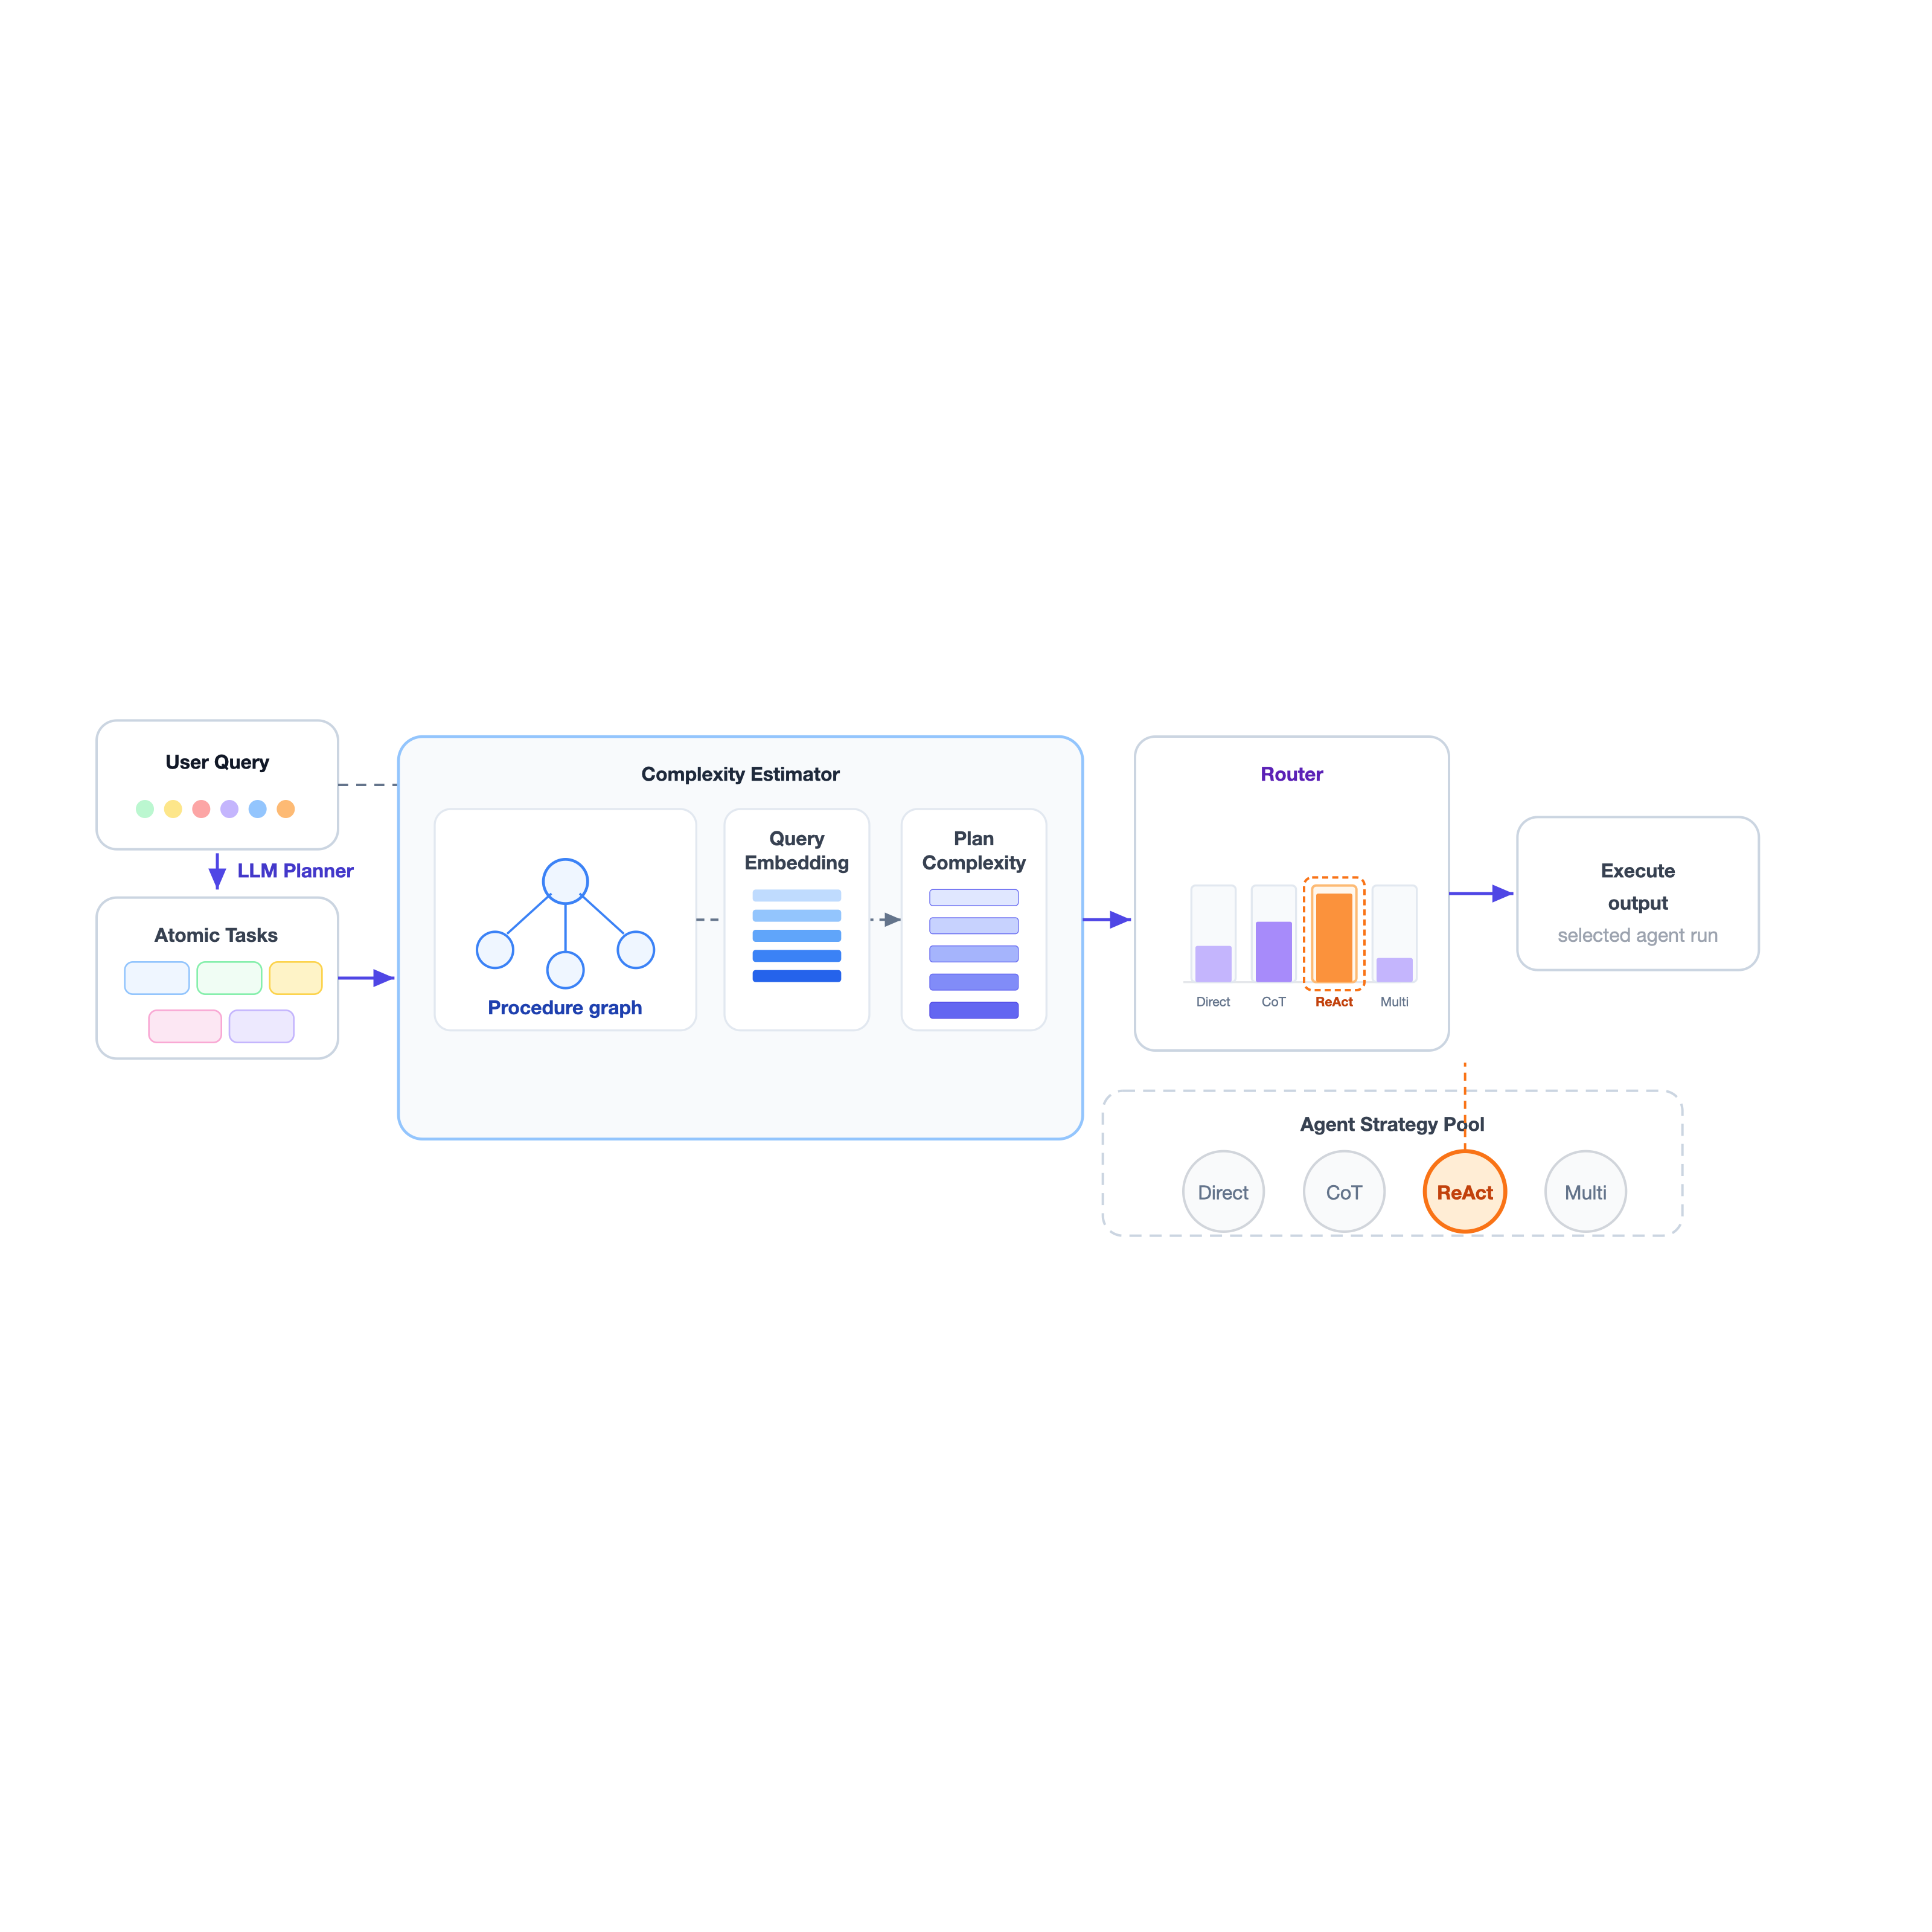
\includegraphics[width=\linewidth]{figures/qce_router_architecture.png}%
        }{%
          \IfFileExists{figures/qce_router_architecture.pdf}{%
            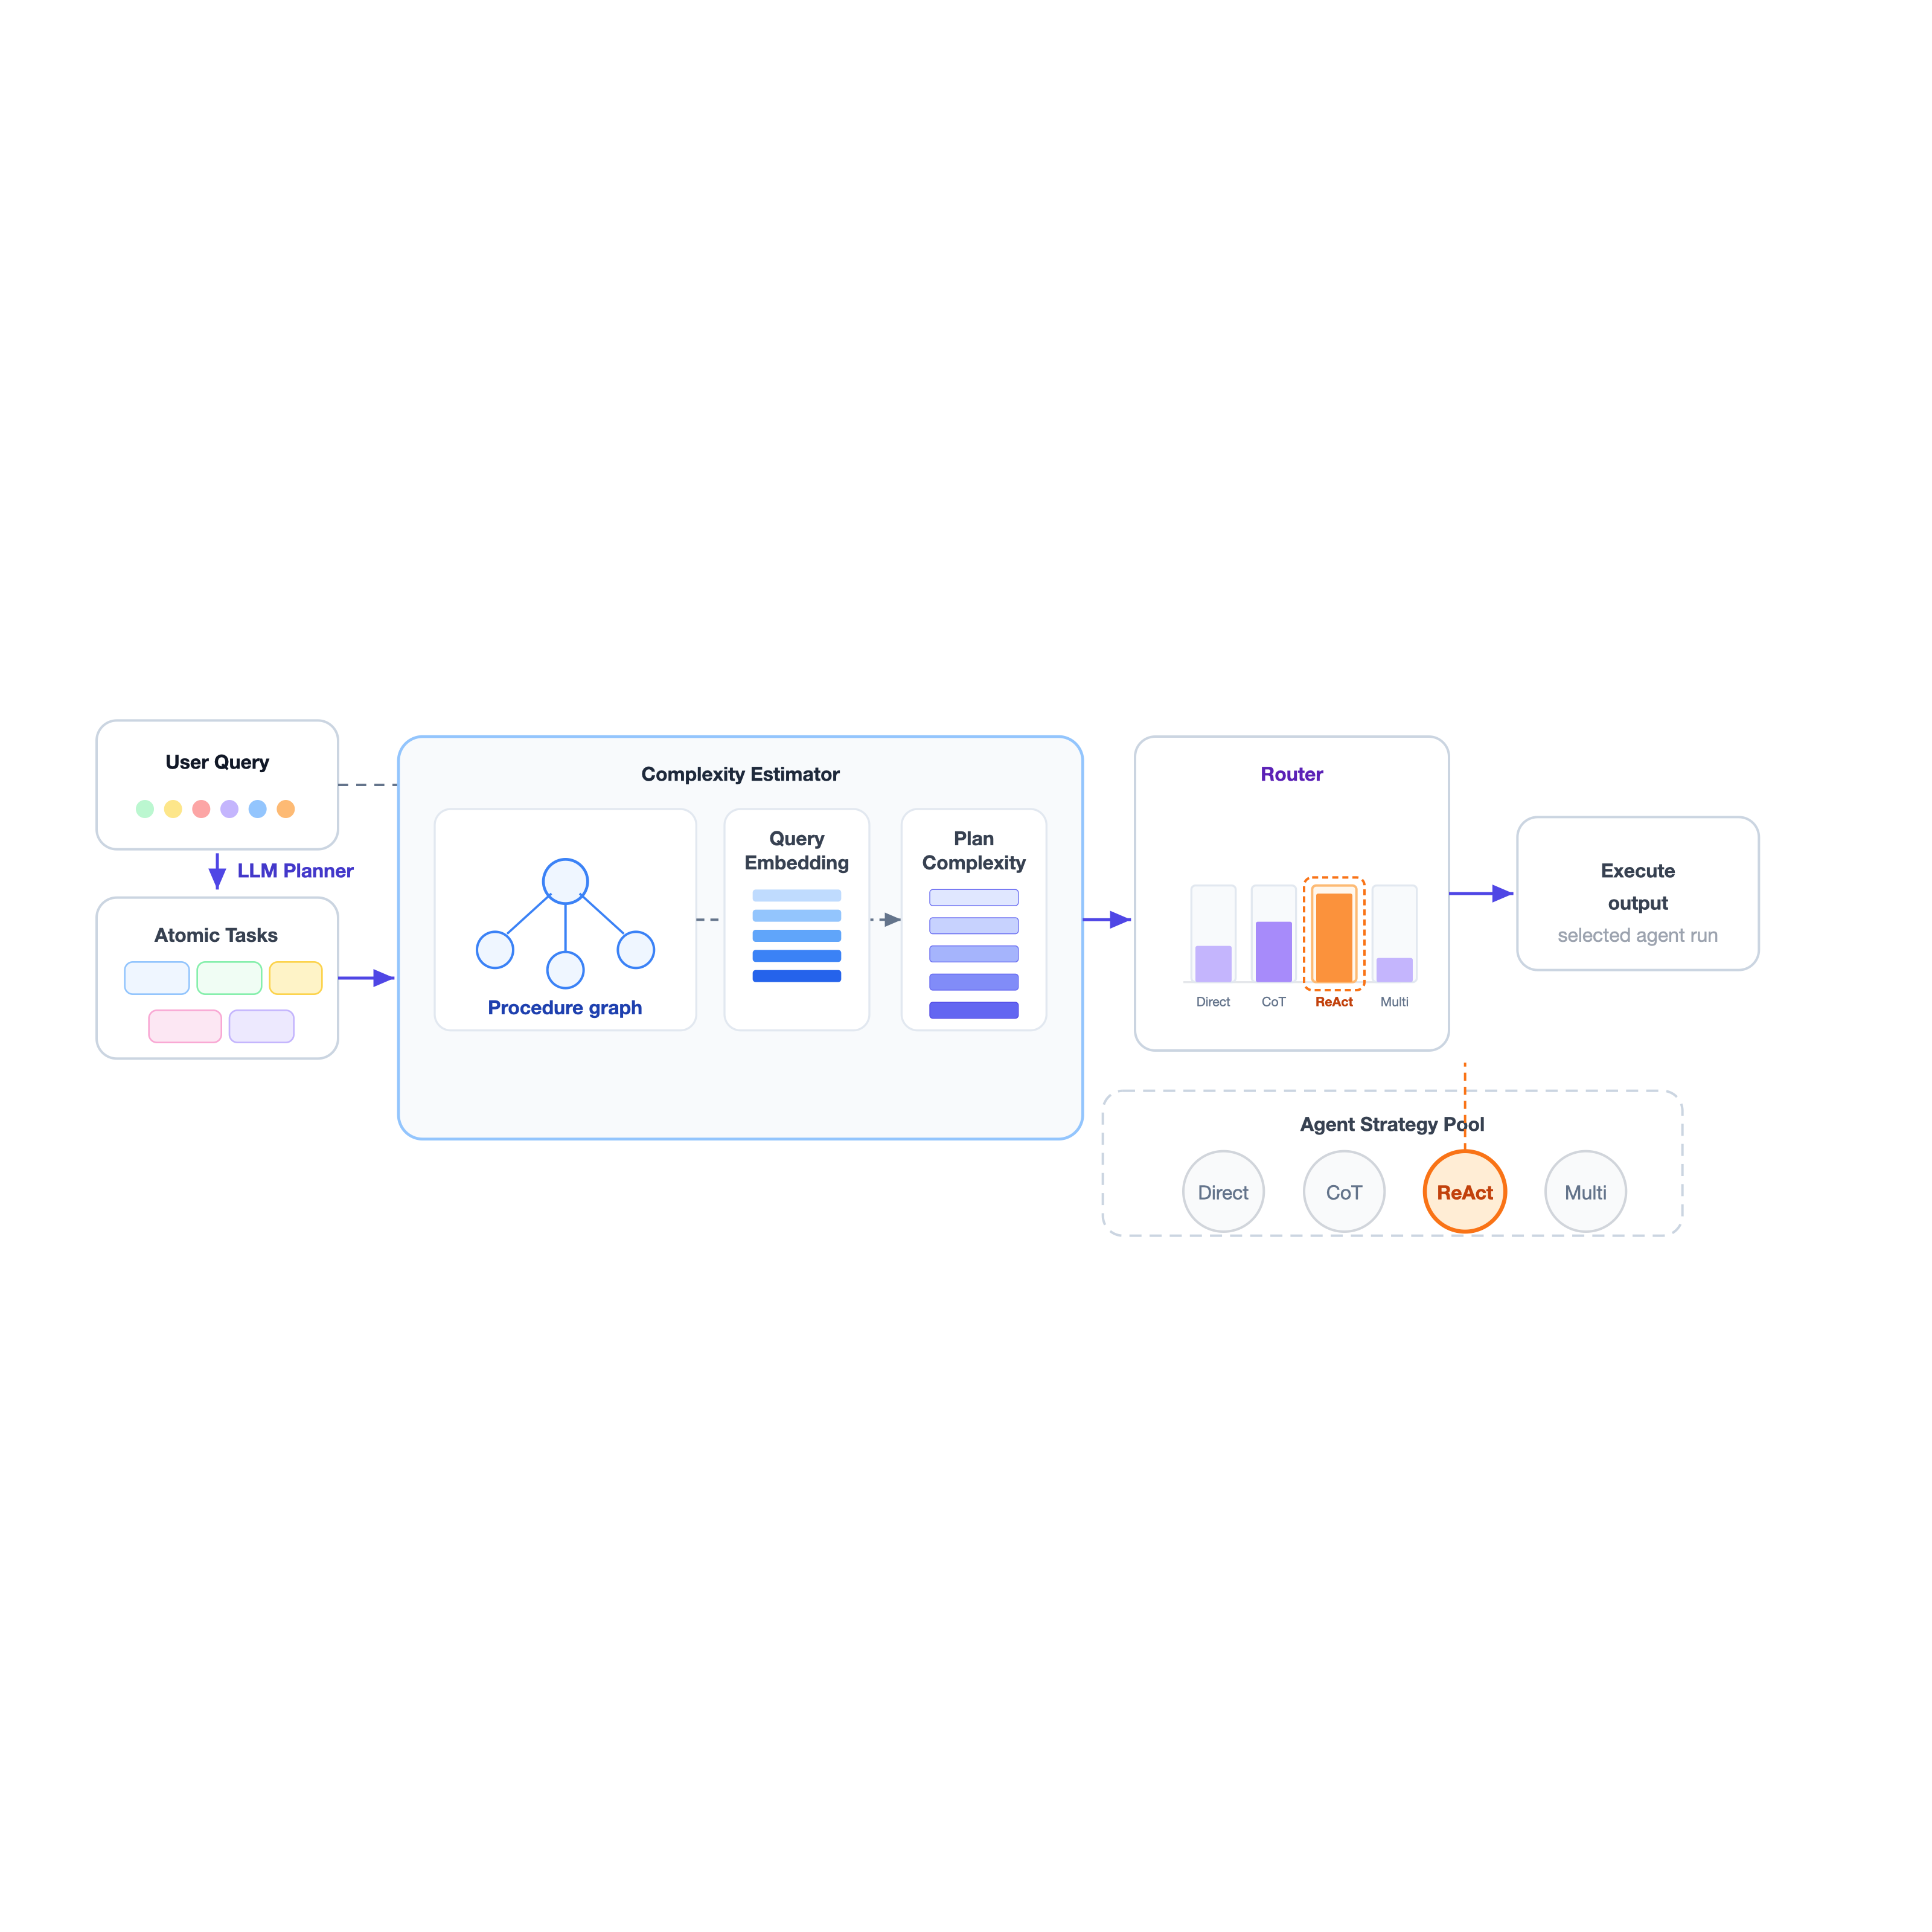
\includegraphics[width=\linewidth]{figures/qce_router_architecture.pdf}%
          }{%
            \fbox{\parbox[c][1.1in][c]{0.92\linewidth}{\centering\small
              Run \texttt{python -m research.figures} $\rightarrow$
              \texttt{results/reports/figures/fig2\_method\_overview.png}.}}%
          }%
        }%
      }%
    }%
  }
  \caption{System architecture of Adaptive Agent Routing (AAR).
    \textbf{Planning:} an LLM planner decomposes query~$q$ into atomic subtasks and a
    procedure graph $G_q=(V,E)$ (Eq.~\ref{eq:method-procedure-graph}).
    \textbf{Complexity estimation:} QCE maps the plan to $\mathbf{z}(q)\in\mathbb{R}^5$;
    query semantics are encoded in parallel as $\psi(q)$ and fused with complexity as
    $\phi(q)=[\mathbf{z}(q);\psi(q)]$ (Eq.~\ref{eq:method-phi}).
    \textbf{Routing and execution:} the router predicts $p_\theta(a\mid\phi(q))$ from
    $\phi(q)$, selects $\hat{a}(q)=\arg\max_{a\in\mathcal{A}} p_\theta(a\mid\phi(q))$
    (Eq.~\ref{eq:method-argmax}) over
    $\mathcal{A}=\{\texttt{raw},\texttt{cot},\texttt{react},\texttt{multiagent}\}$, and
    runs only the chosen agent strategy.
    Offline training minimizes $\mathrm{KL}\bigl(p^\star(\cdot\mid q)\,\|\,p_\theta(\cdot\mid\phi(q))\bigr)$
    on cost-soft targets $p^\star$ (Eqs.~\ref{eq:cost-soft}--\ref{eq:method-kl}).}
  \label{fig:pipeline}
\end{figure}

\subsection{Query Complexity Estimation}
\label{sec:method-qce}

\paragraph{Motivation.}
Queries with similar wording may require very different reasoning procedures.
ReAct-style tool use tends to help when a plan demands retrieval and external tools;
chain-of-thought often suffices when inference is reasoning-intensive but retrieval-light.
Semantic embeddings alone cannot distinguish these procedural requirements because they
do not observe the anticipated solution structure.

\paragraph{Design.}
We introduce an LLM \emph{planner} that decomposes $q$ into a structured execution plan,
represented as a directed acyclic \emph{procedure graph}
\begin{equation}
  G_q=(V,E).
  \label{eq:method-procedure-graph}
\end{equation}
Vertices correspond to atomic subtasks with types \emph{retrieve}, \emph{reason},
\emph{compute}, \emph{verify}, and \emph{select}; directed edges encode dependency and
execution order among subtasks.
$G_q$ is an intermediate artifact for complexity estimation---not a router input and not
an entity-centric knowledge graph.

\paragraph{Formalization.}
The Query Complexity Estimator (QCE) maps $(G_q,\text{plan})$ to a five-dimensional vector
\begin{equation}
  \mathbf{z}(q)=\bigl(z_1(q), z_2(q), z_3(q), z_4(q), z_5(q)\bigr)^\top\in\mathbb{R}^5.
  \label{eq:method-complexity-vector}
\end{equation}
Table~\ref{tab:complexity-dims} summarizes the semantics of each dimension.
Algorithm~\ref{alg:qce} gives the graph-based estimation procedure; feature definitions,
normalization, and term weights are in Appendix~\ref{app:features}.
Decomposition prompts for the procedure planner are in Appendix~\ref{app:decompose-prompts}
(Figure~\ref{fig:decompose-prompt-suite});
agent execution prompts for the four routed strategies are in Appendix~\ref{app:agent-prompts};
a worked GAIA example (planner JSON $\rightarrow$ $G_q$ $\rightarrow$ $\mathbf{z}(q)$) is in
Appendix~\ref{app:gaia-worked-example} (Figure~\ref{fig:gaia-dag-example}).

\begin{table}[t]
  \centering
  \footnotesize
  \setlength{\tabcolsep}{3pt}
  \caption{Query complexity dimensions estimated by QCE.}
  \label{tab:complexity-dims}
  \begin{tabular}{@{}p{0.32\linewidth}p{0.62\linewidth}@{}}
    \toprule
    Dimension & Description \\
    \midrule
    $z_1$ (structural) &
      Estimated procedural depth and branching complexity of the plan \\
    $z_2$ (reasoning) &
      Multi-step inference and reasoning requirements \\
    $z_3$ (evidence) &
      Retrieval and evidence aggregation demand \\
    $z_4$ (tool) &
      Expected dependence on external tools and actions \\
    $z_5$ (coordination) &
      Degree of subtask interaction and orchestration difficulty \\
    \bottomrule
  \end{tabular}
\end{table}

\paragraph{Procedure.}
QCE builds a repaired procedure DAG from the planner output, extracts graph- and plan-level
statistics, normalizes them with train-fitted caps, and aggregates normalized terms into
$\mathbf{z}(q)\in[0,1]^5$ (Table~\ref{tab:complexity-dims}; Appendix~\ref{app:features}).

\begin{algorithm}[t]
  \caption{Graph-aware query complexity estimation (QCE)}
  \label{alg:qce}
  \small
  \begin{algorithmic}[1]
    \Require Query $q$; LLM plan $P$ with atomic subtasks $\mathcal{T}$
    \Ensure Complexity vector $\mathbf{z}(q)\in\mathbb{R}^5$
    \State Build repaired procedure DAG $G_q=(V,E)$ from $\mathcal{T}$
    \State Extract graph and plan statistics $\mathbf{f}=\Phi(G_q,P)$
    \State Normalize $\mathbf{f}$ using train-fitted caps (Appendix~\ref{app:features})
    \State Aggregate normalized terms into $\mathbf{z}(q)=(z_1,\ldots,z_5)^\top$
    \State \Return $\mathbf{z}(q)$
  \end{algorithmic}
\end{algorithm}

\paragraph{Benefit.}
QCE provides complementary procedural signals that are unavailable from semantic embeddings
and can be combined with them for routing (\S\ref{sec:representation-analysis}).

\subsection{Complexity--Semantic Routing Representation}
\label{sec:method-representation}

\paragraph{Motivation.}
Complexity alone does not capture lexical and topical variation in $q$.
Semantic embeddings alone do not capture tool use, retrieval structure, or multi-step
orchestration implied by the plan.
Effective routing therefore requires both signals.

\paragraph{Design.}
We form a fixed pre-inference feature vector by concatenating procedural complexity with
a semantic query representation.

\paragraph{Formalization.}
\begin{equation}
  \phi(q)=\big[\mathbf{z}(q);\,\psi(q)\big],
  \label{eq:method-phi}
\end{equation}
where $\psi(q)$ denotes a low-dimensional semantic embedding of $q$.
The representation hypothesis is that procedural complexity and semantic content provide
complementary information for routing.
Table~\ref{tab:feature-composition} summarizes the production feature groups.
The embedding projection dimension was selected on the validation split via ablation over
$\{8,16,32,64\}$ and fixed at $16$ for all reported experiments
(Appendix~\ref{app:additional-analyses}).
At inference the router consumes $\phi(q)$ only; no message passing is performed on $G_q$.

\begin{table}[t]
  \centering
  \caption{Production routing feature composition (pre-inference).}
  \label{tab:feature-composition}
  \begin{tabular}{lc}
    \toprule
    Feature group & Dimensions \\
    \midrule
    Complexity vector $\mathbf{z}(q)$ & 5 \\
    Embedding projection $\psi(q)$ & 16 \\
    Total $\phi(q)$ & 21 \\
    \bottomrule
  \end{tabular}
\end{table}

\paragraph{Benefit.}
Complexity captures procedural requirements, while embeddings capture lexical and topical
information.
\S\ref{sec:representation-analysis} isolates each signal: complexity-only ($\mathbf{z}$),
embedding-only ($\psi$), and their fusion $\phi(q)$.
Complexity-only underperforms embedding-only on regret, yet the fused representation
outperforms both---planner-derived complexity is complementary rather than sufficient alone.

\subsection{Cost-Soft Supervision}
\label{sec:method-supervision}

\paragraph{Motivation.}
The central hypothesis is that supervision quality is more important than classifier capacity
when multiple strategies are simultaneously correct.
Hard supervision forces a single winner even when multiple agent strategies answer correctly.
For example, both \texttt{cot} and \texttt{react} may achieve $r_a(q)=1$ while differing
substantially in cost.
Collapsing such queries to one hard label discards cost information that routing should
exploit.
Existing hard-label and utility-softmax schemes either collapse to one winner or distribute
mass over all strategies; AAR instead distributes target mass over \emph{successful} strategies
only, weighted by execution cost.

\paragraph{Utility (oracle and regret).}
Eq.~\ref{eq:utility} defines utility $U_a(q)=r_a(q)-\lambda c_a(q)$ for the utility oracle
$a^\star(q)$, hard labels, and regret evaluation.
It does \emph{not} define the cost-soft training targets: those are constructed separately from
$\mathcal{C}(q)$ below.

\paragraph{Successful strategy set.}
Let $\mathcal{C}(q)=\{a\in\mathcal{A}: r_a(q)=1\}$ denote the successful strategies for
query~$q$ (Eq.~\ref{eq:correct-set}).
Table~\ref{tab:cost-soft-cases} summarizes how $p^\star(\cdot\mid q)$ is constructed from
$\mathcal{C}(q)$.

\begin{table}[t]
  \centering
  \footnotesize
  \setlength{\tabcolsep}{3pt}
  \renewcommand{\arraystretch}{1.12}
  \caption{Cost-soft label construction by oracle outcome (training only).}
  \label{tab:cost-soft-cases}
  \begin{tabular}{@{}p{0.31\linewidth}p{0.27\linewidth}p{0.36\linewidth}@{}}
    \toprule
    Scenario & Successful set $\mathcal{C}(q)$ & Target $p^\star(\cdot\mid q)$ \\
    \midrule
    None & $\emptyset$ & Excluded from training \\
    One (e.g.) & $\{\texttt{react}\}$ & One-hot on $\mathcal{C}(q)$ \\
    Multiple (e.g.) & $\{\texttt{cot},\texttt{react}\}$ &
      Cost-soft on $\mathcal{C}(q)$ only (Eq.~\ref{eq:cost-soft}) \\
    \bottomrule
  \end{tabular}
\end{table}

\paragraph{Cost-soft target.}
For $a\in\mathcal{C}(q)$ with $|\mathcal{C}(q)|\ge 2$, targets follow Eq.~\ref{eq:cost-soft},
with $p^\star(a\mid q)=0$ for $a\notin\mathcal{C}(q)$.
If $|\mathcal{C}(q)|=1$, $p^\star$ is one-hot; if $|\mathcal{C}(q)|=0$, the query is excluded
from soft training.
Unlike utility-softmax targets, unsuccessful strategies always receive zero probability mass;
cost-soft distributes mass only over $\mathcal{C}(q)$, with lower-cost successes receiving
higher target weight through $\exp(-\tau c_a(q))$.
Label temperature $\tau$ governs the target distribution and is distinct from utility weight
$\lambda$ (Appendix~\ref{app:hyperparameters}).

\paragraph{Benefit.}
Cost-soft supervision preserves information about multiple successful agent strategies while
encouraging preference toward lower-cost solutions.

\subsection{Router Learning}
\label{sec:method-train}

\paragraph{Motivation.}
The router must predict cost-aware strategy preferences from $\phi(q)$ before any agent
strategy is executed, using only oracle supervision $(r_a(q),c_a(q))$ recorded on the routing
benchmark for training.

\paragraph{Design.}
We learn a parametric distribution $p_\theta(a\mid\phi(q))$ over $a\in\mathcal{A}$ by
minimizing divergence to the cost-soft targets $p^\star(\cdot\mid q)$.

\paragraph{Formalization.}
\begin{equation}
  \mathcal{L}(\theta)=\mathbb{E}_q\bigl[
    \mathrm{KL}\bigl(p^\star(\cdot\mid q)\,\|\,p_\theta(\cdot\mid\phi(q))\bigr)
  \bigr],
  \label{eq:method-kl}
\end{equation}
implemented as sample-weighted multiclass cross-entropy.
We evaluate gradient-boosted trees and multinomial logistic regression as representative
tabular classifiers (\S\ref{sec:main-results}).
Classifier choice is treated as an implementation decision rather than a methodological
contribution; the claim is the supervision and features, not the choice of classifier.

\paragraph{Benefit.}
Consequently, the router learns relative preferences among agent strategies rather than a
single hard assignment.

\subsection{Inference}
\label{sec:method-inference}

\paragraph{Routing.}
Given $\phi(q)$, the deployed strategy is
\begin{equation}
  \hat{a}(q)=\arg\max_{a\in\mathcal{A}} p_\theta(a\mid\phi(q)).
  \label{eq:method-argmax}
\end{equation}

\paragraph{Execution.}
Only $\hat{a}$ is executed; the system returns $\hat{y}(q)=\hat{y}_{\hat{a}(q)}(q)$.

\paragraph{Benefit.}
Unlike ensemble approaches, only one agent strategy runs at deployment, preserving latency
and cost efficiency while training still exploits full cost-soft supervision.
